\documentclass[oneside,onecolumn]{article}


\usepackage{blindtext} % Package to generate dummy text throughout this template 

\usepackage[sc]{mathpazo} % Use the Palatino font
\usepackage[T1]{fontenc} % Use 8-bit encoding that has 256 glyphs
\linespread{1.05} % Line spacing - Palatino needs more space between lines
\usepackage{microtype} % Slightly tweak font spacing for aesthetics

\usepackage[english]{babel} % Language hyphenation and typographical rules

\usepackage[hmarginratio=1:1,top=32mm,columnsep=20pt]{geometry} % Document margins
\usepackage[hang, small,labelfont=bf,up,textfont=it,up]{caption} % Custom captions under/above floats in tables or figures
\usepackage{booktabs} % Horizontal rules in tables

\usepackage{lettrine} % The lettrine is the first enlarged letter at the beginning of the text

\usepackage{enumitem} % Customized lists
\setlist[itemize]{noitemsep} % Make itemize lists more compact

\usepackage{titlesec} % Allows customization of titles
\renewcommand\thesection{\Roman{section}} % Roman numerals for the sections
\renewcommand\thesubsection{\roman{subsection}} % roman numerals for subsections
\titleformat{\section}[block]{\large\scshape\centering}{\thesection.}{1em}{} % Change the look of the section titles
\titleformat{\subsection}[block]{\large}{\thesubsection.}{1em}{} % Change the look of the section titles

\usepackage{fancyhdr} % Headers and footers
\pagestyle{fancy} % All pages have headers and footers
\fancyhead{} % Blank out the default header
\fancyfoot{} % Blank out the default footer
% \fancyhead[C]{Running title $\bullet$ May 2016 $\bullet$ Vol. XXI, No. 1} % Custom header text
\fancyfoot[RO,L]{\thepage} % Custom footer text

\usepackage{titling} % Customizing the title section

\usepackage{hyperref} % For hyperlinks in the PDF

\usepackage{romannum} % Roman numbers 
\usepackage{graphicx}
\usepackage{wrapfig}
\graphicspath{ {images/} }
\usepackage{subcaption}
\usepackage{amsmath}
\usepackage{amssymb}
\usepackage{sidecap}

% ----------------------------------------------------------------------------------------
%	TITLE SECTION
% ----------------------------------------------------------------------------------------

\setlength{\droptitle}{-2\baselineskip} % Move the title up

\pretitle{\begin{center}\Huge\bfseries} % Article title formatting
  \posttitle{\end{center}} % Article title closing formatting
\title{Motion planning of a fixed wings Uav through an hybrid approach based on artificial potential
  fields and RRT. } % Article title
\author{%
  \textsc{Edoardo Ghini} \\[1ex] % Your name
  \normalsize \href{mailto:ghiniedoardo@gmail.com}{ghiniedoardo@gmail.com} % Your email address
  \and % Uncomment if 2 authors are required, duplicate these 4 lines if more
  \textsc{Gianluca Cerilli} \\[1ex] % Second author's name
  \normalsize \href{mailto:gianlucer@gmail.com}{gianlucer@gmail.com}\\ % Second author's email address
  \normalsize Dipartimento di Ingegneria dell'Universita di Roma La Sapienza\\
}
\date{\today} % Leave empty to omit a date

\begin{document}

% Print the title
\maketitle
\bigskip
\bigskip
\bigskip
\bigskip
\begin{center}
  \includegraphics[width=0.3\textwidth]{laSapienza}
\end{center}

\newpage
\section{Introduction}

\lettrine[nindent=0em,lines=3]{W}e will present a work made
for an international challenge\footnote{The challenge is the AUVSI-SUAS hosted
  in united states in summer 2018.} that every year involves several accademic teams.\\
This report respects the following structure : \\
in section \Romannum{2}, we will present the problem statement and in section
\Romannum{3} we will give tecnical informations on the hardware at our disposal,
finally in section \Romannum{4}, the adopted solution will be discussed.

\section{Problem Statement}
All the joining teams to the challenge will have to compete on several tasks
concerning on actual problems in the governance of Unmanned Aerial Vehicles.\\
Each team will bring its prototype of UAV on a common flight ground and try to
score the greatest number of points among all the tasks proposed which are:
\begin{enumerate}\centering
\item Autonomous Flight
\item Obstacle Avoidance
\item Object Detection
\item Object Classification
\item Object Localization 
\item Air Delivery
\end{enumerate}


This will be the first partecipation at a competition of this kind for the team
Sapienza, in fact the previous challenges in which our university has already
been involved required a human controlled guidance system.
Therefore the autonomous flight constraint has to be faced without previous
insights on the matter.

\subsection{Starting Points}
The areonautical research department, in the past decade, has spent a big
effort working to an autonomous guidance system, that has been thinkered,
designed and implemented by master students in theyr thesis.\\
This system allows to control the complex aerodynamics of the vehicle from an
higher level of abstraction, its main high level control mode uses a series of
way points that describes a trajectory.\\

\begin{wrapfloat}{figure}{o}{0pt}
  \includegraphics[width=0.3\textwidth]{YAK1}
  \caption{YAK scaled aero model}\label{wrap-fig:1}
\end{wrapfloat} 


In this way the aircraft will likely follow a path made of lines that intersects subsequent waypoints.\\
The system is designed to work on an on-board computer and to communicate with a
ground station that will continuously send to and receive from the judges's
server, telemetrical data and mission objectives.\\
We will use a fixed-wigs radio controlled aircraft model\footnote{It is a scaled
  reproduction (1:3 ratio) of the YAK 112} commonly used in hobby
modeling as shown in Figure~\ref{wrap-fig:1}.


\subsection{Our task}
As atomic part of the team which counts several members coming from an
aeronutical background, we have an uncommon area of expertise that concerns
\textbf{automation} and \textbf{robotics}.\\ So we engaged the autonomous guidance problem that
comprehend also the obstacle avoidance clause.\par
The competition will be organized in such a way that during the various missions
of the challenge each team will receive pose informations about fixed and mobile
obstacles that will be \textbf{virtual}.\\
Then the judges will check the success or failure in avoiding obstacles
according to the \textbf{telemetry} data that they will receive from each team.\\
In other words, we where supposed to design a \textbf{path planning} algorith
that will bring the UAV from a start position to a goal position without
collisions.\\
Additionally we contributed to the integration of the ground control station
with the interoperability protocols that allows an efficient communication with
the judge's server, both for receiving mission information, obstacle position
and sending the telemetry of the aircraft.


\section{Hardware components}
All the components described in this section, left aside the propulsive module,
will work with two different voltages ( around 3 and 5 Volts ). For this reason
two converters have been adopted, in particular the \textit{Tracopower TSR 1-2433
 } and the \textit{Recom R-78B5.0-1.5}.
\subsection{Propulsion}
\begin{wrapfloat}{figure}{o}{0pt}
  \includegraphics[width=0.2\textwidth]{YAK3}
  \caption{DLE55 motor}\label{wrap-fig:2}
\end{wrapfloat} 

The engine chosen is a \textbf{DLE55} (in Figure~\ref{wrap-fig:2} ).
\begin{enumerate}
\item 50 cc monocylinder petrol engine
\item reservoir capable of containing 950cc of petrol
\item Equipped with a 7, 4V LiPo battery
\end{enumerate}


\subsection{On board computing}
The autonomous guidance architecture, implemented in Matlab and Simulink, is
converted in compiled high speed C, Cpp language.\\ It will be run by Arduino Due
and there will be also a Raspberry pi Model 3 that will run a kalman filter in
order to process all signals from sensors.


\begin{wrapfloat}{figure}{o}{0pt}
  \includegraphics[width=0.3\textwidth]{extLoop}
  \caption{External loop}\label{wrap-fig:3}
\end{wrapfloat} 



\subsection{Sensing instruments}
Concerning the sensors which are mounted on the aeromodel we have a GPS
receiver, namely \textit{ Lassen IQ} and an attitude and heading reference
system ( \textit{MTi} model).\\
We also find a pressure and temperature sensor which is a \textit{BMP280} and an
intrestingly complex system to measure the fluid flow velocity (in this case the
fluid measured is the air around the plane body) that is the \textit{Honeywell SSC}.
\subsection{Communication devices}
Ensure secure and continuous communication between the aeromodel and the ground
station is a crucial point, in fact we employed two capable antennas, the
\textit{Xbee Pro S2C}. They will be placed one on the lower body of the aircraf
and the other on the ground.\\
These reliable antennas works at 2.4 GHz and are omnidirectional, they support
an operational range of 1.5 Km and in our case, some extimations made clear to
use a 96 dB gain in the antenna on the ground.

\begin{wrapfloat}{figure}{o}{0pt}
  \includegraphics[width=0.25\textwidth]{intLoop}
  \caption{Internal loop}\label{wrap-fig:4}
\end{wrapfloat} 


\subsection{Auto pilot framework}

The system supports six modes :
\begin{itemize}
\item Boot and pre-flight checklist
\item Calibration of sensor 
\item Ready before mission start
\item Manual guidance
\item Stand by (transition state)
\item Autonomous guidance
\end{itemize}

Talking about the last mode, there are two main approaches supported by the
\textbf{Auto Pilot} : \textit{Vectorial} guidance and \textit{Waypoint-based}
navigation.



The vectorial guidance is controllable through four desired values:
\begin{itemize}
\item \textbf{ALT}: altitude
\item \textbf{RC}: rate of climb (roll angle $\phi$)
\item \textbf{IAS}: velocity
\item \textbf{HDG}: heading (yaw angle $\psi$)
\end{itemize}
An oversemplified conceptual map is shown in Figure~\ref{wrap-fig:3} Figure~\ref{wrap-fig:4}.
\newpage
\section{Hybrid planner}
We implemented two different strategies, since both present some shortcomings
and advantages, we tried to take the best of the two worlds.

\subsection{RRT}

\begin{wrapfloat}{figure}{o}{0pt}
  \includegraphics[width=0.3\textwidth]{rrt}
  \caption{Behaviour of RRT search near obstacles}\label{wrap-fig:5}
\end{wrapfloat} 

RRT (Rapidly-exploring Random Tree) is a probabilistic planner that randomly builds a space-building tree.\\
It has been used offline considering some motion primitives (produced by some specific velocity inputs) to define a path for the UAV, biasing it towards the unexplored areas closest to the goal.
One intresting aspect of this probabilistic approach is that it will eventually
find a way to reach the goal if it exists. In Figure~\ref{wrap-fig:5} we can see
how the algorithm explores all the branches of the tree and expanding unexplored
nodes and discarding colliding ones it will succed to find the path between the
two obstacles.
\subsection{Artificial potentials}
\begin{SCfigure}[]
\centering
\includegraphics[width=0.3\textwidth]{artPotFields}
\caption{Example of the potentials distribution on a map with three obstacles
    and the goal on the lower right corner}
\label{wrap-fig:6}
\end{SCfigure}

Artificial Potential Fields (APF) have been considered for two main reasons:
\begin{itemize}
\item the world can be approximated to a "world of spheres" (since there are cylindrical obstacles that we consider in 2D), that prevents the UAV entering the basin of attraction of some local minima
\item when the UAV faces an obstacle, RRT must expand many branches before getting around it. This leads to a significant slowdown
\end{itemize}

\begin{figure}
\centering
   {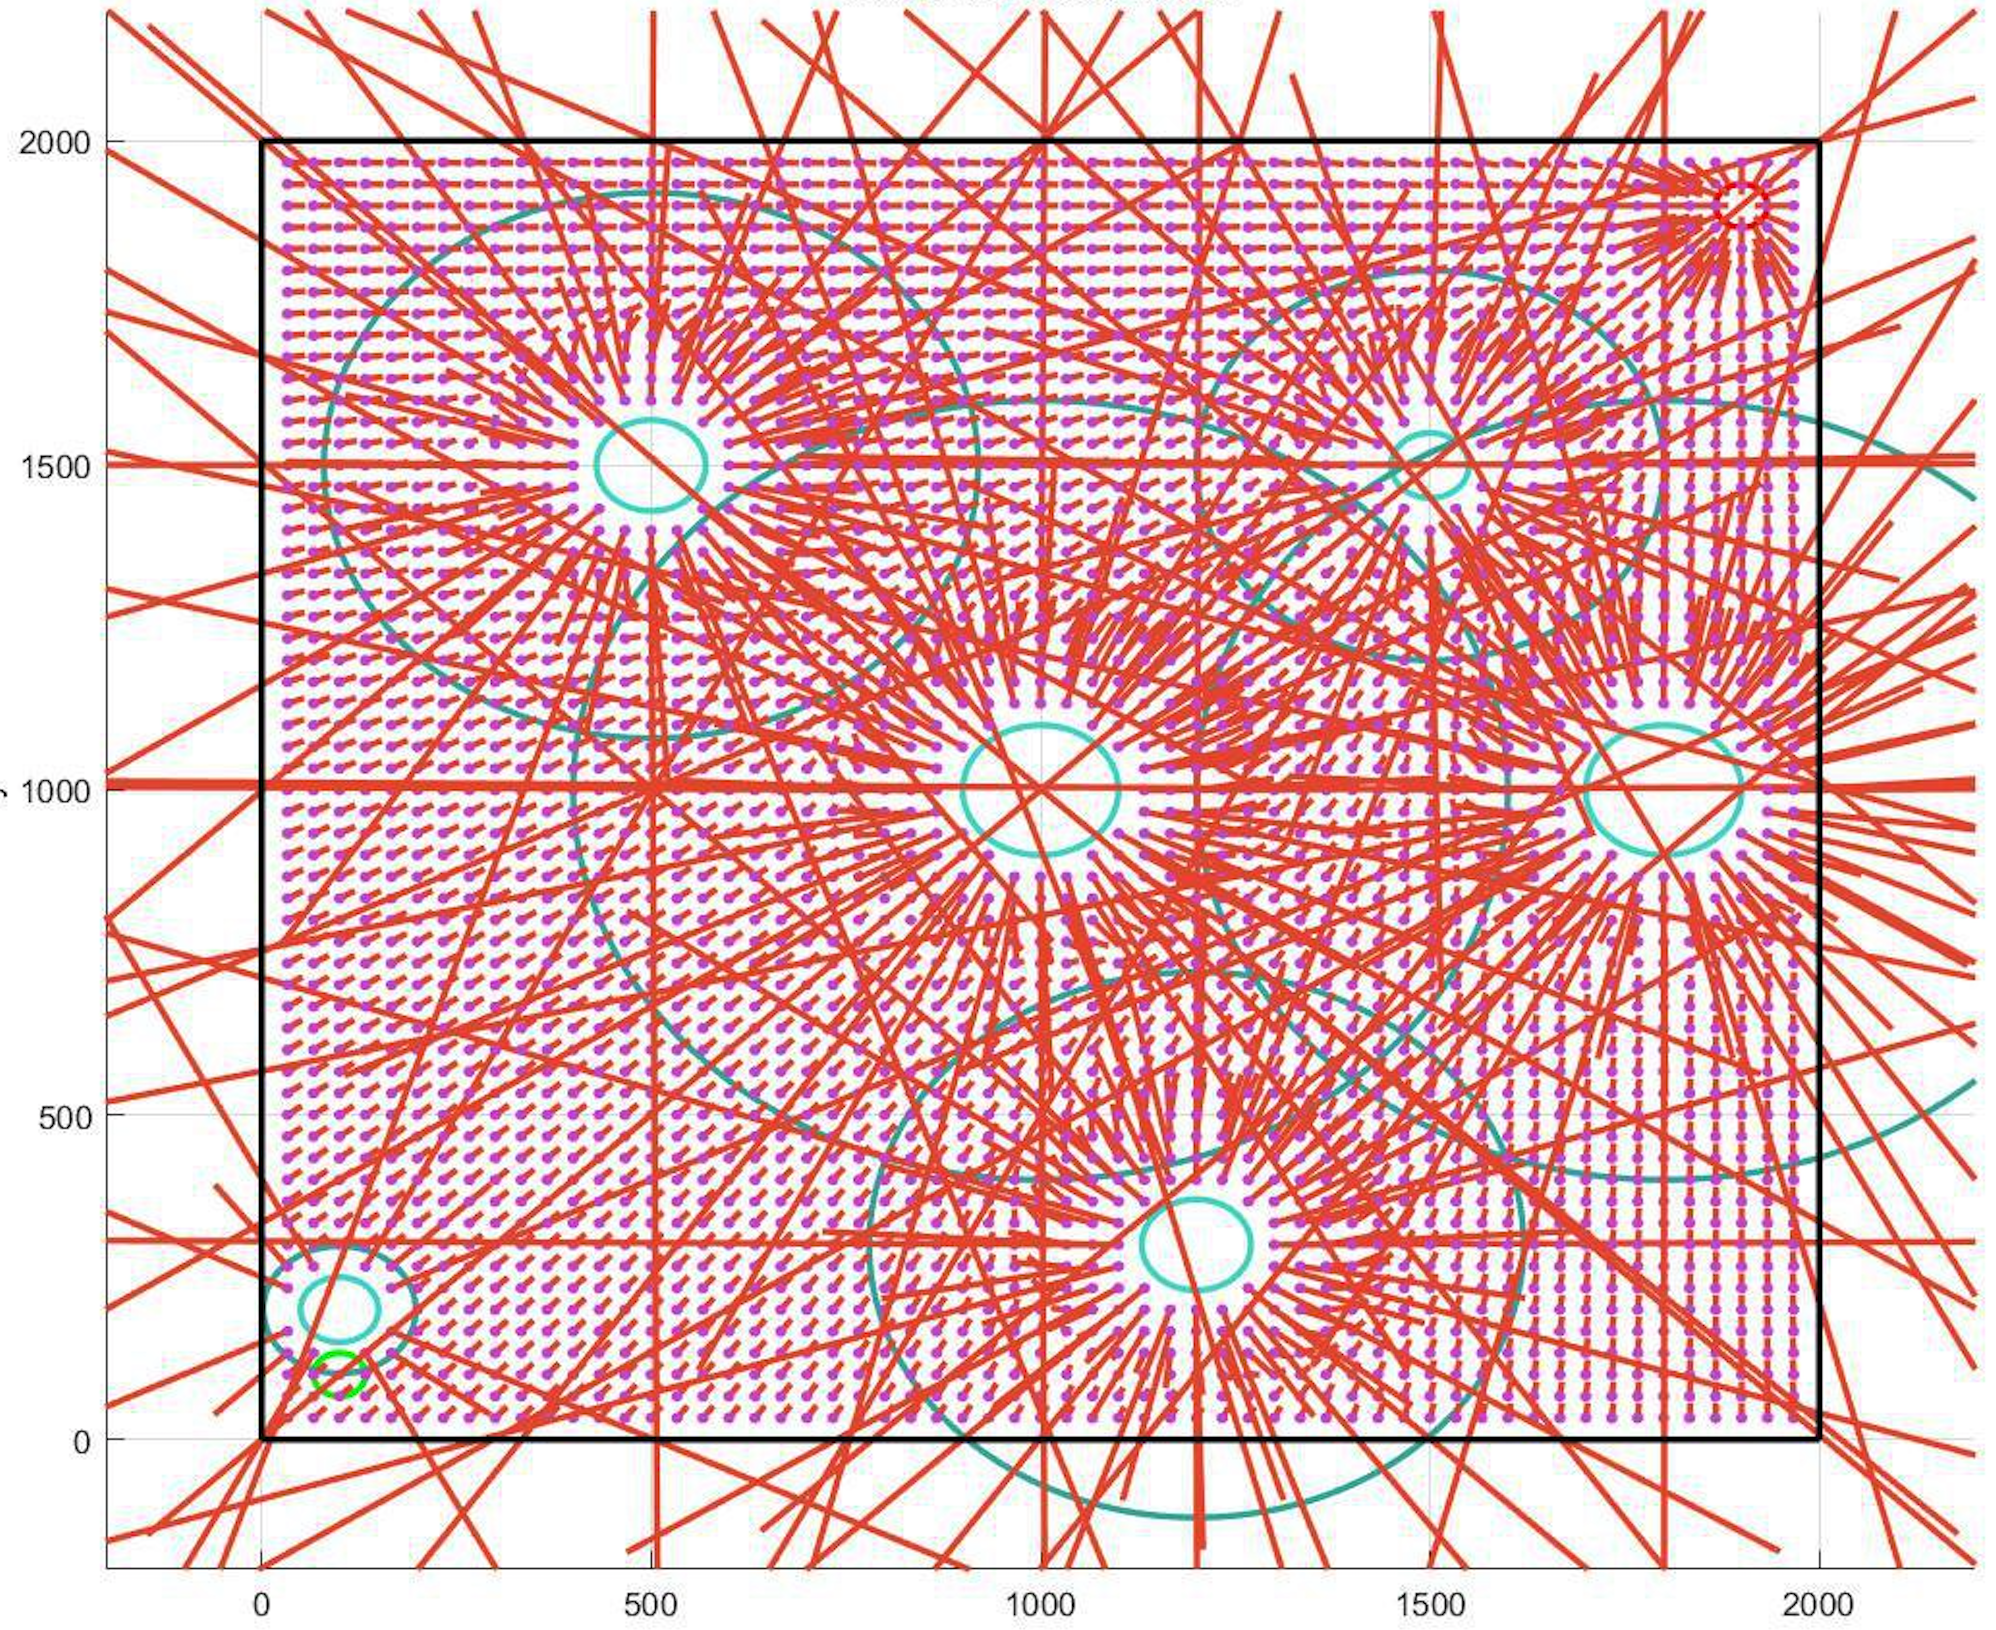
\includegraphics[width=.45\textwidth]{noVort}} \quad
   {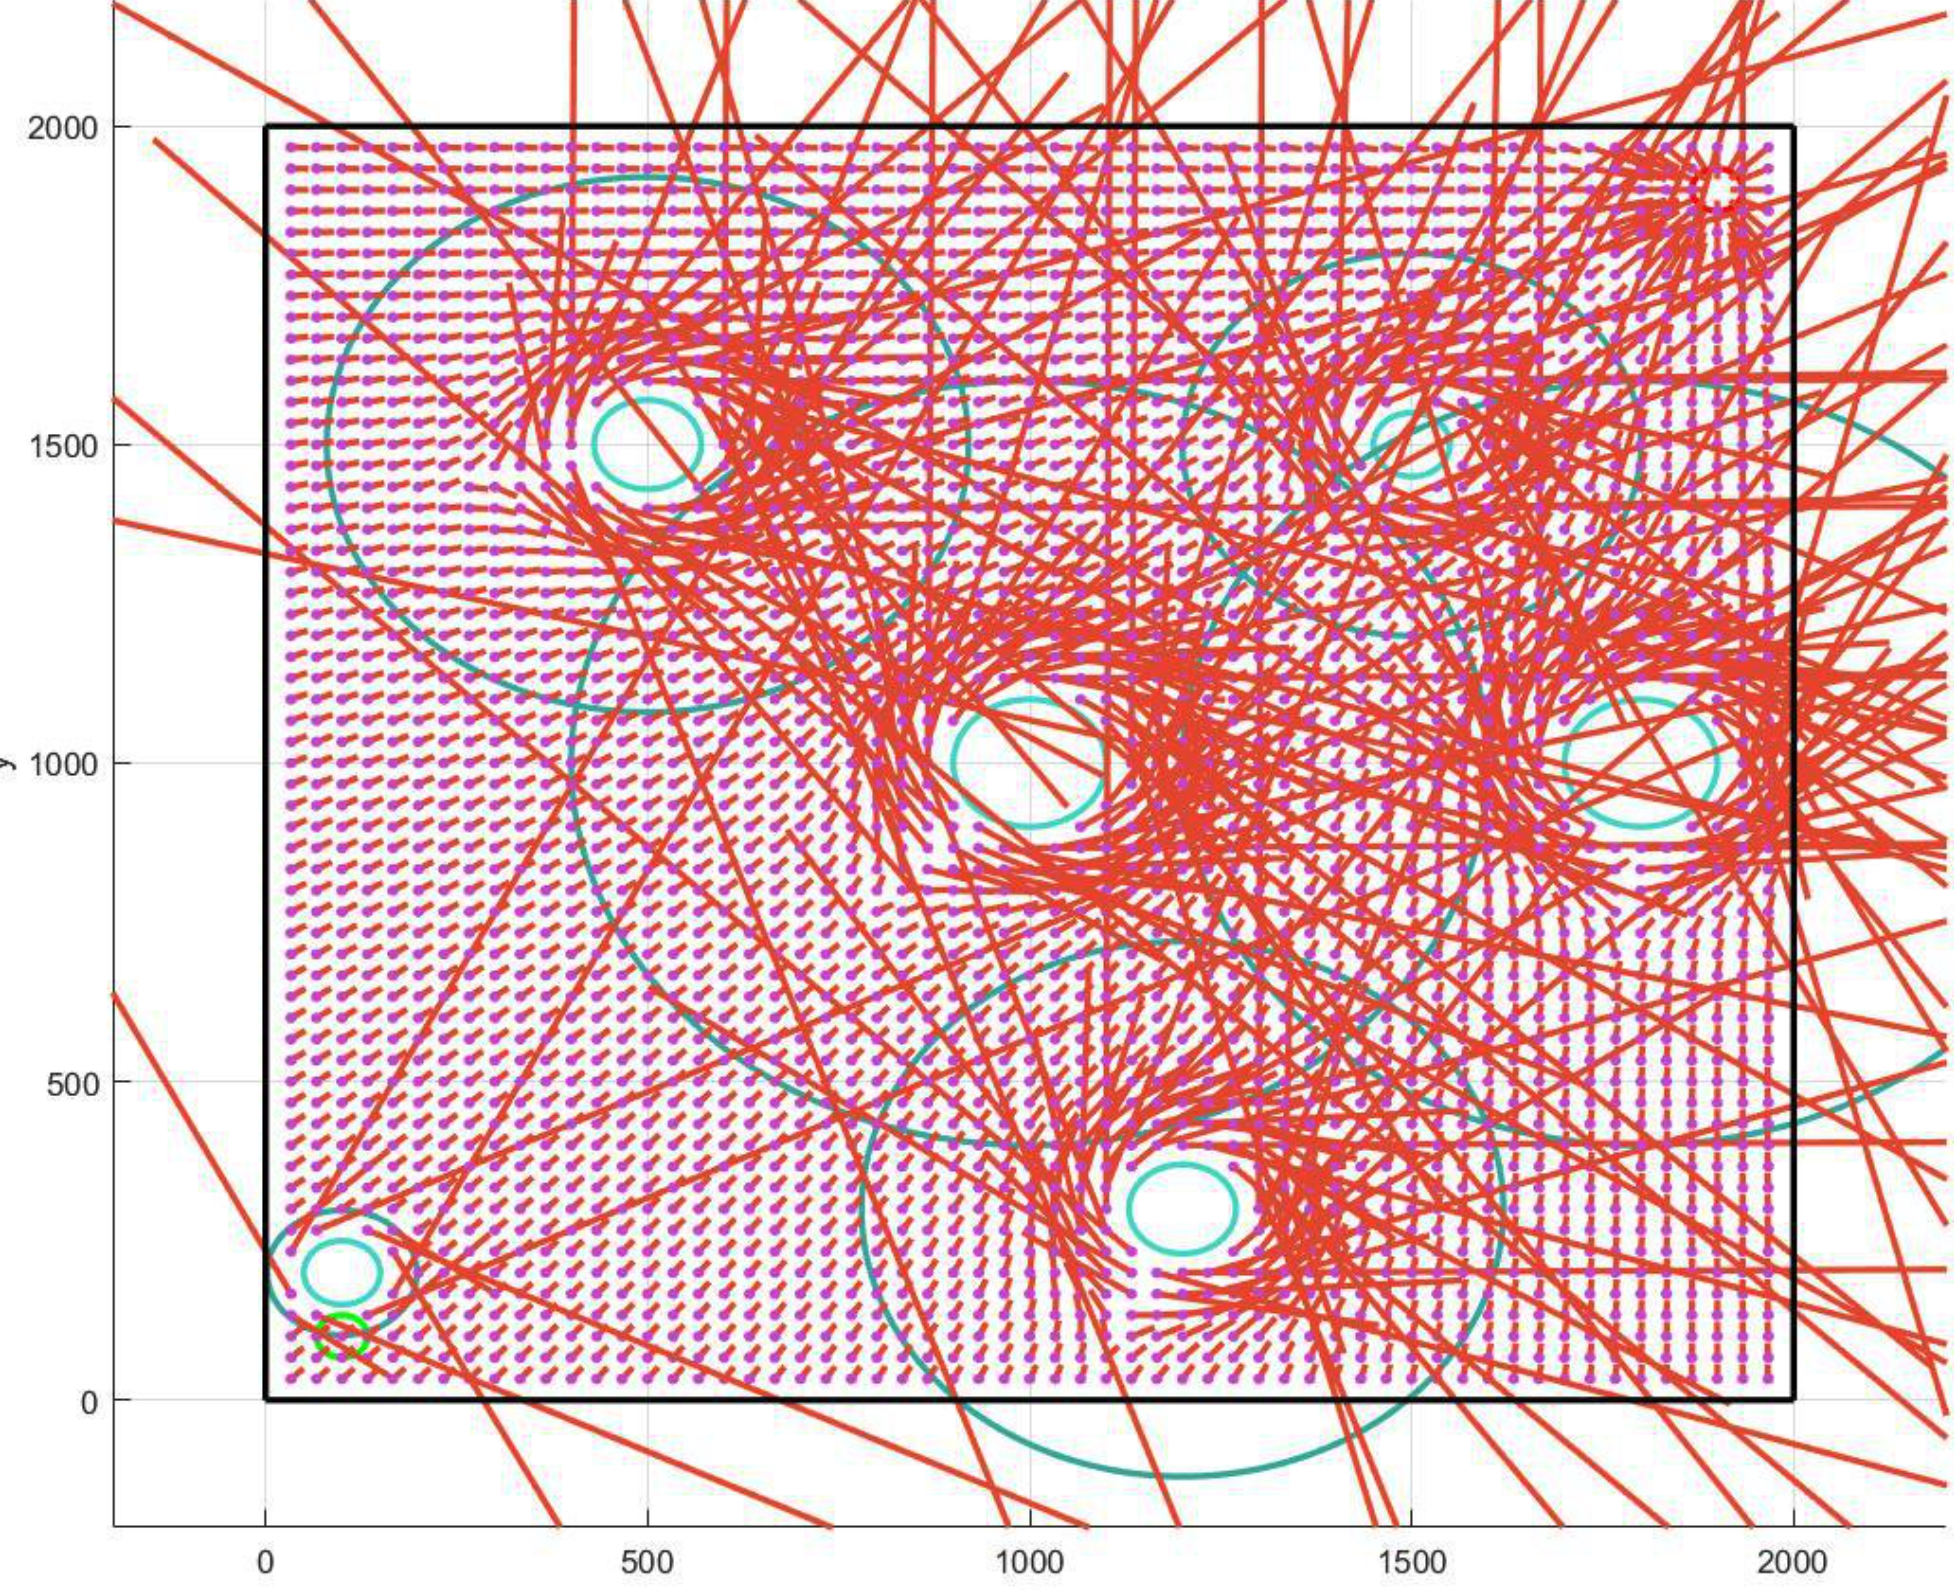
\includegraphics[width=.45\textwidth]{vortex}} \\
\caption{Map with vectors pointing in the gradient of the artificial potential
  fields: the difference between the two images is that in the right the vortex
  was implemented while in the left wasn't.}
\label{fig:subfig1}
\end{figure}

Using APF the UAV can react as soon as entering the range of influence of the
obstacle, with a smooth movement. This result has been made possible thanks to
the implementation of vortex fields, replacing repulsive actions with actions
forcing the robot to get around each obstacles, in practice generating a
tangential gradient that follows a circle around the obstacle that will guide
the aircraft avoiding harmful gradients pointing against the natural direction
of motion as shown in Figure~\ref{fig:subfig1}.
\subsection{Implementation}
\begin{figure}
\centering
   {\includegraphics[width=.45\textwidth]{execution}} \quad
   {\includegraphics[width=.45\textwidth]{finalPath}} \\
\caption{On the left is shown the dynamic execution of the planning algorithm,
  on the right there is the path followed by the UAV after that the plannig has been completed.}
\label{fig:subfig2}
\end{figure}
We consider the kinematic model of a fixed-wing UAV flying at a constant
altitude.
So, we can neglect the pitch angle, obtaining:\\
\begin{center}
\[
  \dot{x} = u_{v}cos{\theta} \psi
\]
\[
  \dot{y} = u_{v}sin{\theta} \psi
\]
\[
  \dot{\psi} = - \frac{g}{u_{v}} tan \phi 
\]
\[
  \dot{\phi} = u_{\phi}
\]
\end{center}

in which the tangential velocity $u_{v}$ and roll rate $u_{\phi}$ are the control inputs.

\section{Interoperability integration}
In order to achieve an efficient communication we where nearly obliged to make
use of the python \textbf{API} written by the challenge organizers. In this way the
communication can be handled with \textit{asyncronous} \textbf{HTTP} requests between each team
client and the judge's server.\\
Since our team has choosen a code base in MATLAB, we implemented an interface
that allows to invoke the API functions directly from MATLAB code.\\
Then every significative data received will be saved in a compatible file ( in
our case in a .mat file) that will be read and used in the execution cycle of the Auto
Pilot infrastructure.



\bigskip
\bigskip
\bigskip
\bigskip
\bigskip
\bigskip
\bigskip
\bigskip
\bigskip
\bigskip
\bigskip
\bigskip
\bigskip
\bigskip
\bigskip



\section{Conclusion}
In the end, we consider the experience that we have made a good way to face
problems spreaded on a large spectrum.\\
In retrospection, it was a very time-taxing challenge and in our opinion it
demands a lot more time and effort from the team to be able to confront the
other teams around the world.\\
In such a way they already  come from past years experinces and results,
and they alse have an accumulated knowledge about the issues that we, instead, have had to
solve for the first time.\\
We hope that this work could be a base for the next challenges of our university
and that the competition in June will score good results.
\end{document}
